\documentclass[a4paper, 12pt]{article}

\usepackage[top=1in, bottom=1in, left=1in, right=1in]{geometry}

\usepackage{tikz}
\newcommand*\circled[1]{\tikz[baseline=(char.base)]{
            \node[shape=circle,draw,inner sep=2pt] (char) {#1};}}
\usetikzlibrary{positioning, shapes.geometric, arrows.meta, arrows}
\usepackage{enumitem}

\usepackage{float}
% To make subfirgures
\usepackage{caption, subcaption}

\usepackage{cancel}
\usepackage{braket}

\usepackage[top=1in, bottom=1in, left=1in, right=1in]{geometry}
\usepackage{amsmath, amssymb, amsthm, graphicx}
\usepackage{mathtools} % aboxed, among other things
\usepackage{xfrac}

% Base equation numbering on the current subsubsection
\numberwithin{equation}{subsubsection}


% More space in matrices. Example usage: \pmatrix{}[1.5] for 1.5 times spacing
\makeatletter
\renewcommand*\env@matrix[1][\arraystretch]{%
  \edef\arraystretch{#1}%
  \hskip -\arraycolsep
  \let\@ifnextchar\new@ifnextchar
  \array{*\c@MaxMatrixCols c}}
\makeatother


\usepackage{cancel}

\usepackage{empheq}
\usepackage{fancybox}
\usepackage{multicol}
\usepackage{mathtools}
\usepackage{braket}
\usepackage{siunitx}

\usepackage{enumitem}
\setlength{\parindent}{0pt}

\usepackage{bm}
\usepackage{xcolor}
\usepackage{colortbl}

\usepackage{array, booktabs}
\usepackage{dsfont}

\usepackage{calligra}
\usepackage{mathrsfs}

\usepackage{empheq}
\usepackage{fancybox}
\usepackage{multicol}

\usepackage[parfill]{parskip}
\setlength{\parindent}{0pt}
\usepackage{tcolorbox}
\usepackage{tikz-cd}
\usepackage{mathtools}

\usepackage{array}
\usepackage{dsfont}

\usepackage{color}
\usepackage{hyperref}
\hypersetup{
    colorlinks=true, %set true if you want colored links
    linktoc=all,     %set to all if you want both sections and subsections linked
    linkcolor=blue,  %choose some color if you want links to stand out
}

\title{Fluid Mechanics Notes}
\author{Marcus Koschmieder Krogsgaard}

\begin{document}

\maketitle

\section{Introduction and Flow Kinematics}
\subsection{Streamlines, pathlines and streaklines}

A \textbf{streamline} is a curve that is locally tangent to the velocity field at every point. This requirement can be expressed as:
\begin{align}
	dx/u = dy/v = dz/w
\end{align}
Streamlines can be found by using this relation to establish one or more differential equations.

A \textbf{pathline} is the curve obtained by following the trajectory of a single particle over time. To find the pathlines, use this relationship between the derivatives of the position of the particle and the velocity field
\begin{align}
	\frac{d}{dt} \mathbf{x}_\text{particle} &= \mathbf{u}
\end{align}
And integrate with the initial conditions $\mathbf{x}(t_0) = (x_0, y_0, z_0)$ to get
\begin{align}
	\mathbf{x}_\text{particle}(t) &= \mathbf{x}_\text{particle}(t, x_0, y_0, z_0, t_0) \label{eq:introduction_pathline_diff_eq}
\end{align}

A \textbf{streakline} is the curve obtained by connecting all fluid particles that will ever pass through a given point in space. The equations for streaklines are obtained in a similar way to those for pathlines
\begin{align}
	\mathbf{x}_\text{streakline}(t) &= \mathbf{x}_\text{streakline}(t, x_0, y_0, z_0, t_0) \label{eq:introduction_streakline_diff_eq}
\end{align}
The important distinction between eqs. (\ref{eq:introduction_pathline_diff_eq}) and (\ref{eq:introduction_streakline_diff_eq}) is that $t_0$ is kept fixed in (\ref{eq:introduction_pathline_diff_eq}), since we are only considering one particle (the one that is released at $t_0$). In (\ref{eq:introduction_streakline_diff_eq}), we vary $t_0$ to obtain the trajectories of all particles that will ever pass through $(x_0, y_0, z_0)$.

\subsection{Lagrangian and Eulerian descriptions}
\begin{itemize}
	\item \textbf{Lagrangian:} follows the trajectory of a \textit{specific particle} over time (particle description of motion)
	\item \textbf{Eulerian:} describes the motion of an arbitrary particle \textit{at a particular location and specific instant of time} (field description of motion)
\end{itemize}

\textbf{Motivation for the Eulerian description}:

The Eulerian approach solves the question: \textit{Given a velocity field $\mathbf{V}(x, y, z, t)$; find the acceleration $\mathbf{a}_p$ of a fluid particle at $(x, y, z, t)$.}

We start by noting that the instantaneous velocity of the particle is given by the velocity field at $(x, y, z, t)$
\begin{align}
	\mathbf{u}_p(t) &= \mathbf{V} (x, y, z, t)
\end{align}
At $t + dt$ the particle will have a new instantaneous velocity
\begin{align}
	\mathbf{u}_p(t + dt) &= \mathbf{V} (x + dx, y + dy, z + dz, t + dt)
\end{align}
The infinitesimal change in the particle's velocity is given by the chain rule
\begin{align}
	d\mathbf{u}_p &= \frac{\partial \mathbf{V}}{\partial x} dx + \frac{\partial \mathbf{V}}{\partial y} dy + \frac{\partial \mathbf{V}}{\partial z} dz + \frac{\partial \mathbf{V}}{\partial t} dt
\end{align}
So the total acceleration of the particle is
\begin{align}
	\mathbf{a}_p &= \frac{d\mathbf{V}}{dt} \\
	&= \frac{\partial \mathbf{V}}{\partial x} u + \frac{\partial \mathbf{V}}{\partial y} v + \frac{\partial \mathbf{V}}{\partial z} w + \frac{\partial \mathbf{V}}{\partial t}
\end{align}
At this point is is useful to introduce the so-called \textit{material derivative}, or \textit{substantial derivative}
\begin{align}
	\frac{D}{D t} &= u \frac{\partial }{\partial x} + v \frac{\partial }{\partial y} + w \frac{\partial }{\partial z} + \frac{\partial}{\partial t} \\
	&= \frac{\partial }{\partial t} + (\mathbf{V} \cdot \nabla) \label{eq:introduction_material_derivative}
\end{align}
Which allows us to write the acceleration of the particle as
\begin{align}
	\mathbf{a}_p = \frac{D \mathbf{V}}{D t} &= (\mathbf{V} \cdot \nabla) \mathbf{V} + \frac{\partial \mathbf{V}}{\partial t} \label{eq:introduction_eulerian_flow}
\end{align}
The first term represents movement due to convection (the steady part of the flow) and the time derivative term represents the local acceleration due to unsteadiness in the flow. Eq. (\ref{eq:introduction_eulerian_flow}) is the equation used to compute the acceleration of fluid particles in the Eulerian description.


\subsection{Kinematics}
\begin{figure}[h!]
    \centering
    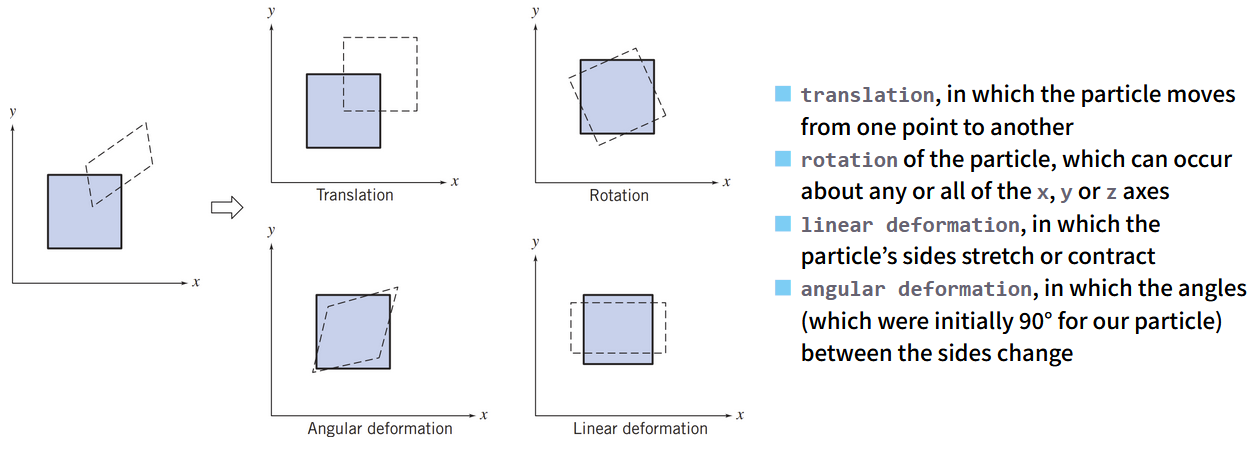
\includegraphics[width=1\linewidth]{img/introduction/fluid_segment_motion.png}
    \caption{Various types of motion of a 2D fluid segment.}
    \label{fig:introduction_fluid_segment_motion}
\end{figure}

Fig. \ref{fig:introduction_fluid_segment_motion} illustrates the four types of motion that are possible for a 2D fluid segment. Any time evolution of a fluid segment will be a combination of these four types of motion.

\subsubsection{Translation}

The translation of an individual fluid particle is connected with the velocity field via eq. (\ref{eq:introduction_eulerian_flow})
\begin{align*}
	\mathbf{a}_p = \frac{D \mathbf{V}}{D t} &= (\mathbf{V} \cdot \nabla) \mathbf{V} + \frac{\partial \mathbf{V}}{\partial t}
\end{align*}
Since this can be solved to find the translation of an individual particle, it may be used to describe how fluid segments are translated as well. We see that translatory motion depends only on the acceleration of particles in the flow.

\subsubsection{Rotation}

The rotation of a particle in a flow can be modelled with a vector $\mathbf{\omega} = (\omega_x, \omega_y, \omega_<)$ whose components are the angular velocities associated with rotation about the three coordinate axes. Fig. \ref{fig:introduction_fluid_rotation_and_deformation} a) and b) show how a square fluid segment undergoes some deformation and rotation during a time interval $\Delta t$. The deformation is described by the translation displacements $\Delta \eta$ and $\Delta \xi$ as well as the angular displacements $\Delta \alpha$ and $\Delta \beta$. Note that $\Delta \alpha$ is positive, while $\Delta \beta$ is negative, since we use the convention that counterclockwise rotation is the positive direction of rotation.
 
Fig. \ref{fig:introduction_fluid_rotation_and_deformation} shows 
\begin{figure}[h!]
    \centering
    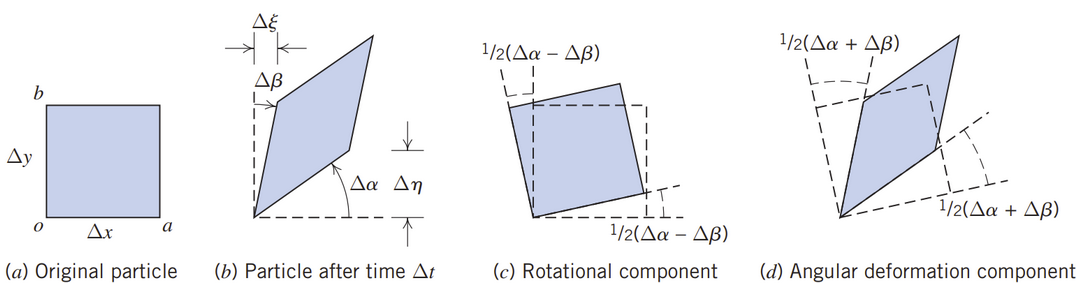
\includegraphics[width=1\linewidth]{img/introduction/introduction_fluid_rotation_and_deformation.png}
    \caption{ }
    \label{fig:introduction_fluid_rotation_and_deformation}
\end{figure}

The segment's rigid body rotation (the rotational motion) can be found by taking the average of the two angular displacements, see fig. \ref{fig:introduction_fluid_rotation_and_deformation} c). The minus sign in $\frac{\Delta \alpha - \Delta \beta}{2}$ is due to the fact that we are taking the average in the counterclockwise direction, and the counterclockwise rotation of $ob$ is $-\Delta \beta$.

We will also need to find the translational displacements $\Delta \eta$ and $\Delta \xi$. To do so, we will consider the situation where all of the displacements and angles involved in the problem are small. Then we can Taylor expand the velocity field $\mathbf{V}$ to get
\begin{align}
	V_x(b) &= V_x(o) + \frac{\partial V_x}{\partial y} \Delta y
\end{align}
So the $x$-displacement of $b$ will be $\left(V_x(o) + \frac{\partial V_x}{\partial y} \Delta y\right) \Delta t$. To find $\Delta \xi$ we must subtract the displacement of the origin which is $V_x(o) \Delta t$. That leaves us with
\begin{align}
	\Delta \xi &= \frac{\partial V_x}{\partial y} \Delta y \Delta t
\end{align}
The same argument can be used to obtain
\begin{align}
	\Delta \eta &= \frac{\partial V_y}{\partial x} \Delta x \Delta t
\end{align}
In our small-displacement approximation, we can write the angular displacements as
\begin{align}
	\Delta \alpha &= \frac{\Delta \eta}{\Delta x} \\
	\Delta \beta &= \frac{\Delta \xi}{\Delta y}
\end{align}
Leading to the following result:
\begin{align}
	\frac{1}{2} \frac{(\Delta \alpha - \Delta \beta)}{\Delta t}   = \frac{1}{2} \frac{\left(\frac{\Delta \eta}{\Delta x} - \frac{\Delta \xi}{\Delta y}\right)}{\Delta t} = \frac{1}{2} \frac{\left(\frac{\partial V_y}{\partial x} \Delta t - \frac{\partial V_x}{\partial y} \Delta t\right)}{\Delta t}
\end{align}
To find the angular velocity about the $z$-axis, we take the limit $\Delta t \rightarrow 0$
\begin{align}
	\omega_z &= \frac{1}{2} \left(\frac{\partial V_y}{\partial x} - \frac{\partial V_x}{\partial y}\right)
\end{align}
This is the $z$-component of the curl of the velocity field (multiplied by a factor of $1/2$). The same argument can be applied to fluid segments in the $yz$- and $xz$-planes, so we conclude that
\begin{align}
	\mathbf{\omega} &= \frac{1}{2} \nabla \times \mathbf{V} = \mathbf{\zeta}
\end{align}
Where we've introduced the vorticity $\mathbf{\zeta} = 2 \mathbf{\omega} = \nabla \times \mathbf{V}$ to get rid of the factor of $1/2$.

\subsubsection{Angular Deformation}

Fig. \ref{fig:introduction_fluid_segment_motion} d) illustrates how the angular deformation component is the sum of the individual angular displacements $\Delta \alpha + \Delta \beta$ (find out where the factor of $1/2$ comes from!)

We can repeat the last steps of our previous calculation to see that the total angular deformation in the $xy$-plane $R_{xy}$ is given by	
\begin{align}
	R_{xy} &= \lim_{\Delta t \rightarrow 0} \frac{1}{2} \frac{(\Delta \alpha + \Delta \beta)}{\Delta t} \\
	&= \frac{1}{2} \left(\frac{\partial V_y}{\partial x} + \frac{\partial V_x}{\partial y}\right)
\end{align}
And by the same reasoning
\begin{align}
	R_{yz} &= \frac{1}{2} \left(\frac{\partial V_z}{\partial y} + \frac{\partial V_y}{\partial z}\right) \\
	R_{xz} &= \frac{1}{2} \left(\frac{\partial V_z}{\partial x} + \frac{\partial V_x}{\partial z}\right)
\end{align}

So angular deformation and rotation is described by the rotation tensor $R_{ij} = \frac{1}{2} \left(\frac{\partial V_i}{x_j} - \frac{\partial V_j}{x_i} \right)$

\subsubsection{Linear Deformation}
Linear deformation (deformation that preserves right angles) in the $x_i$-direction is only possible if $\frac{\partial V_i}{x_i} \neq 0$. This quantity represents the longitudinal strain rate in the $x_i$-direction. Unlike other types of deformation, linear deformation may lead to changes in volume given by the volume dilation rate
\begin{align}
	\text{volume dilation rate} &= \frac{\partial V_x}{\partial x} + \frac{\partial V_y}{\partial y} + \frac{\partial V_z}{\partial z} = \nabla \cdot \mathbf{V}
\end{align}

A flow is \textit{incompressible} if the volume dilation is zero $\nabla \cdot \mathbf{V} = 0$. 

We see that linear deformation is described by the strain rate tensor $S_{ij} = \frac{1}{2} \left(\frac{\partial V_i}{x_j} + \frac{\partial V_j}{x_i} \right)$

\subsubsection{Tensor Representation of Deformation}
To model the deformation that fluid segments undergo, we need to consider the gradient of the velocity field (we have just seen that the derivatives of the velocity field are needed to describe the various types of fluid segment motion).

The gradient of the velocity field is a tensor with the following entries
\begin{align}
	\nabla \mathbf{V} &= A_{ij} = \partial_i v_j
\end{align}
It is a known result from tensor calculus that \textit{any} tensor can be decomposed into a symmetric and an antisymmetric part. This is easily shown by writing the tensor $T_{ij}$ in a clever way and adding and subtracting the transpose $T_{ji}$
\begin{align*}
	T_{ij} &= \frac{1}{2} T_{ij} + \frac{1}{2} T_{ij} \\
	&= \frac{1}{2} T_{ij} + \frac{1}{2} T_{ji} + \frac{1}{2} T_{ij} - \frac{1}{2} T_{ji} \\
	&= \frac{1}{2} (T_{ij} + T_{ji}) + \frac{1}{2} (T_{ij} - T_{ji})
\end{align*}
It can be shown that the first term is symmetric and the second is antisymmetric. Applying this result to $A_{ij}$, we see that
\begin{align}
	A_{ij} &= \frac{1}{2} (\partial_i v_j + \partial_j v_i) + \frac{1}{2} (\partial_i v_j - \partial_j v_i)
\end{align}
Considering the components of the symmetric and antisymmetric parts leads to the revelation that the symmetric part is the angular rotation tensor and the antisymmetric part is the strain rate tensor (both encountered in the previous sections)
\begin{align}
	A_{ij} &= \frac{1}{2} E_{ij} + \frac{1}{2} S_{ij}
\end{align}



\section{From Newton's Second Law to the Navier-Stokes Equations}

\subsection{Conservation of Mass in an arbitrary Control Volume}
\textbf{Important distinction:} For the purposes of this section, a \textit{material volume} is the volume occupied by a specific collection of fluid particles, while a \textit{control volume} is any arbitrary volume whose contents may change over time. In other words, the \textit{material volume} changes as the fluid particles move, while the control volume can be chosen arbitrarily.

Consider a (possible time-dependent) material volume $V(t)$ in a flowing fluid with the fluid density $\rho(\mathbf{x}, t)$. Then the statement of conservation of mass can be expressed as
\begin{align}
	\frac{d}{dt} \int_{V(t)} \rho(\mathbf{x}, t) dV = 0 \label{eq:N2_NS_volume_mass_conservation}
\end{align}
Now we apply Reynolds transport theorem which makes the following statement (add derivation of this to the mathematics section)
\begin{align}
	\frac{d}{dt} \int_{V(t)} \rho(\mathbf{x}, t) dV = \int_{V(t)} \frac{\partial \rho(\mathbf{x}, t)}{\partial t} d V + \int_{A(t)} \rho(\mathbf{x}, t) \mathbf{b} \cdot \mathbf{n} dA \label{eq:N2_NS_reynolds_transport_theorem}
\end{align}
Note that $A(t)$ is the surface of the material volume $V(t)$. Furthermore, $\mathbf{b}$ is the velocity of $A$ and $\mathbf{n}$ is the outward normal vector of $A$. Applying Reynolds transport theorem to the conservation of mass leads to
\begin{align}
	\int_{V(t)} \frac{\partial \rho(\mathbf{x}, t)}{\partial t} d V + \int_{A(t)} \rho(\mathbf{x}, t) \mathbf{u}(\mathbf{x}, t) \cdot \mathbf{n} dA = 0 \label{eq:N2_NS_reynolds_on_mass_conservation}
\end{align}
Where we have labeled the velocity of the material surface with $\mathbf{u}(\mathbf{x}, t)$, to distinguish it from the control surface we will introduce in a moment.

So far, we have been considering a \textit{material volume}. However, a statement of conservation of mass for an arbitrary \textit{control volume} is highly desirable. As a first step, we apply Reynolds transport theorem to the conservation of mass in the control volume $V^*$
\begin{align}
	\frac{d}{dt} \int_{V^*(t)} \rho(\mathbf{x}, t) dV - \int_{V^*(t)} \frac{\partial \rho(\mathbf{x}, t)}{\partial t} d V - \int_{A^*(t)} \rho(\mathbf{x}, t) \mathbf{b} \cdot \mathbf{n} dA = 0 \label{eq:N2_NS_control_volume_mass_reynolds_theorem}
\end{align}
Since the control volume is arbitrary, we can choose $V^*$ such that $V^*(t) = V(t)$ and $A^*(t) = A(t)$ at the specific time $t$ we are considering. Since $V^*$ and $V$ are only instantaneously coincident the time derivative terms $\frac{d}{dt} \int \rho dV$ are not necessarily equal at $t$. However, the terms that don't contain time derivatives \textit{are} equal at the time $t$. Combining this knowledge with eq. (\ref{eq:N2_NS_control_volume_mass_reynolds_theorem}) gives us
\begin{align}
	\int_{V(t)} \frac{\partial \rho(\mathbf{x}, t)}{\partial t} d V = - \int_{A(t)} \rho(\mathbf{x}, t) \mathbf{u}(\mathbf{x}, t) \cdot \mathbf{n} dA = \int_{V^*(t)} \frac{\partial \rho(\mathbf{x}, t)}{\partial t} d V = - \int_{A^*(t)} \rho(\mathbf{x}, t) \mathbf{u}(\mathbf{x}, t) \cdot \mathbf{n} dA
\end{align}
We can use this to replace the second term in eq. (\ref{eq:N2_NS_control_volume_mass_reynolds_theorem})
\begin{align}
	\frac{d}{dt} \int_{V^*(t)} \rho(\mathbf{x}, t) dV - \int_{V^*(t)} \frac{\partial \rho(\mathbf{x}, t)}{\partial t} d V - \int_{A^*(t)} \rho(\mathbf{x}, t) \mathbf{b} \cdot \mathbf{n} dA &= 0\\
	\Leftrightarrow \frac{d}{dt} \int_{V^*(t)} \rho(\mathbf{x}, t) dV + \int_{A^*(t)} \rho(\mathbf{x}, t) \mathbf{u}(\mathbf{x}, t) \cdot \mathbf{n} dA - \int_{A^*(t)} \rho(\mathbf{x}, t) \mathbf{b} \cdot \mathbf{n} dA &= 0 \\
	\Leftrightarrow \frac{d}{dt} \int_{V^*(t)} \rho(\mathbf{x}, t) dV + \int_{A^*(t)} \rho(\mathbf{x}, t) (\mathbf{u}(\mathbf{x}, t) - \mathbf{b}) \cdot \mathbf{n} dA &= 0 \label{eq:N2_NS_control_volume_mass_conservation}
\end{align}
Eq. (\ref{eq:N2_NS_control_volume_mass_conservation}) is the statement of mass conservation for an arbitrary control volume. Note that $\mathbf{u}$, the velocity of the material surface, and $\mathbf{b}$, the velocity of the control surface, must be observed in the same coordinate system (the same frame of reference).

\subsection{The Continuity Equation}
Let's dive deeper into the material volume mass conservation statement to derive a differential form of mass conservation. Recall Gauss' theorem, which states that \textit{for any $C^1$ vector field $\mathbf{F}$ defined on an open and bounded subset $V \subset \mathbf{R}^n$}
\begin{align}
	\int_V \nabla \cdot \mathbf{F} dV &= \int_{A} \mathbf{F} \cdot \mathbf{n} dA
\end{align}
Where $A = \partial V$ is the boundary of the volume $V$. Applying Gauss' theorem to the surface integral in eq. (\ref{eq:N2_NS_reynolds_on_mass_conservation}) gives
\begin{align}
	\int_{V(t)} \frac{\partial \rho (\mathbf{x}, t)}{\partial t} + \nabla \cdot (\rho(\mathbf{x}, t) \mathbf{u}(\mathbf{x}, t)) dV = 0
\end{align}
Since this must be true for every volume, the integrand must vanish at every point in space, which finally leaves us with
\begin{align}
	\frac{\partial \rho (\mathbf{x}, t)}{\partial t} + \nabla \cdot (\rho(\mathbf{x}, t) \mathbf{u}(\mathbf{x}, t)) = 0
\end{align}
The first term is the rate of change of the mass density, while the second term is the divergence of the mass density flux. The continuity equation can be re-written using the following product rule
\begin{align*}
	\nabla \cdot (\rho \mathbf{u}) = \rho \nabla \cdot \mathbf{u} + (\mathbf{u} \cdot \nabla) \rho
\end{align*}
And the definition of the material derivative (\ref{eq:introduction_material_derivative})
\begin{align*}
	\frac{D \rho}{D t} = \frac{\partial \rho}{\partial t} + \mathbf{u} \cdot \nabla \rho
\end{align*}
To obtain the so-called \textit{continuity equation}
\begin{align}
	\frac{1}{\rho} \frac{D \rho}{D t} + \nabla \cdot \mathbf{u} = 0 \label{eq:N2_NS_continuity_eq}
\end{align}
Note that for \textit{incompressible} flow the material derivative vanishes and the continuity equation becomes
\begin{align}
	\nabla \cdot \mathbf{u} = 0 \label{eq:N2_NS_incompressible_continuity_eq}
\end{align}
A flow is incompressible if the density of the fluid is constant throughout the flow. Eq. (\ref{eq:N2_NS_incompressible_continuity_eq}) is sometimes considered the definition of incompressibility, since it is equivalent to the condition that the density is constant.

\subsection{Conservation of Momentum in an arbitrary Control Volume}
Newton's second law applied to a material volume $V(t)$ looks like this
\begin{align}
	\frac{d}{dt} \int_{V(t)} \rho(\mathbf{x}, t) \mathbf{u}(\mathbf{x}, t) dV = \frac{d}{dt} \int_{V(t)} \rho(\mathbf{x}, t) \mathbf{g}dV + \frac{d}{dt} \int_{A(t)} \mathbf{f}(\mathbf{n}, \mathbf{x}, t) dA
\end{align}
Here $\rho \mathbf{u}$ is the momentum per unit volume of flowing fluid, $\mathbf{g}$ is the body force (body forces are forces acting inside the material volume) per unit mass acting on the fluid within $V$ and $\mathbf{f}$ is the surface force per unit area acting on $A$. $\mathbf{n}$ is the outward normal vector on $A$. Applying Reynolds transport theorem (\ref{eq:N2_NS_reynolds_transport_theorem}) gives
\begin{align}
	\int_{V(t)} \frac{\partial}{\partial t} (\rho(\mathbf{x}, t)\mathbf{u}(\mathbf{x}, t)) dV + \int_{A(t)} \rho(\mathbf{x}, t)\mathbf{u}(\mathbf{x}, t) (\mathbf{u}(\mathbf{x}, t) \cdot \mathbf{n}) dA \notag \\
	= \int_{V(t)} \rho(\mathbf{x}, t) \mathbf{g}dV + \int_{A(t)} \mathbf{f}(\mathbf{n}, \mathbf{x}, t) dA
\end{align}
The result for an arbitrary control volume is achieved through the same process as for conservation of mass, so I will just quote the result
\begin{align}
	\int_{V^*(t)} \frac{\partial}{\partial t} (\rho(\mathbf{x}, t)\mathbf{u}(\mathbf{x}, t)) dV + \int_{A^*(t)} \rho(\mathbf{x}, t)\mathbf{u}(\mathbf{x}, t) (\mathbf{u}(\mathbf{x}, t) - \mathbf{b}) \cdot \mathbf{n} dA \notag \\
	= \frac{d}{dt} \int_{V^*(t)} \rho(\mathbf{x}, t) \mathbf{g}dV + \int_{A^*(t)} \mathbf{f}(\mathbf{n}, \mathbf{x}, t) dA \label{eq:N2_NS_momentum_conservation}
\end{align}

\subsection{Tensor Representation of Body and Surface Forces}
Body forces are forces that act internally within the volume $V$ without physical contact. Examples are gravity and electromagnetic forces. Body forces are always distributed throughout the volume and proportional to the total mass (or charge, current, etc.) contained within the volume. Consider the case where the body forces are conservative. In this case, they may be written as the gradient of a potential function $\Phi$
\begin{align}
	\mathbf{g} = - \nabla \Phi, \quad g_i = - \partial_i \Phi
\end{align}

The surface forces in the various coordinate directions may be expressed using the stress tensor $T_{ij}$ and surface normal $\mathbf{n}$
\begin{align}
	\mathbf{f} = \mathbf{n} \cdot \mathbf{T}, \quad f_i = T_{ji} n_j
\end{align}
It can be shown that the stress tensor is symmetric using Cauchy's tetrahedron argument (add this to the mathematics section if you like suffering).

\subsection{Differential form of Momentum Conservation (Cauchy's Equation)}
To obtain a differential form of the momentum conservation equation for a material volume, we apply Gauss' theorem on the surface integrals in eq. (\ref{eq:N2_NS_momentum_conservation})
\begin{align}
	\int_{A(t)} \rho(\mathbf{x}, t)\mathbf{u}(\mathbf{x}, t) (\mathbf{u}(\mathbf{x}, t) - \mathbf{b}) \cdot \mathbf{n} dA &= \int_{V(t)} \nabla \cdot (\rho(\mathbf{x}, t)\mathbf{u}(\mathbf{x}, t)) \mathbf{u}(\mathbf{x}, t) dV = \int_{V(t)} \partial_i (\rho u_i u_j) dV \\
	\int_{A(t)} \mathbf{f}(\mathbf{n}, \mathbf{x}, t) dA &= \int_{A(t)} \mathbf{T} \cdot \mathbf{n} dA = \int_{V(t)} \nabla \cdot \mathbf{T} dV = \int_{V(t)} \partial_i T_{ij} dV
\end{align}
Substituting this into (\ref{eq:N2_NS_momentum_conservation}) and collecting the terms in one volume integral gives:
\begin{align}
	\int_{V(t)} \partial_t (\rho u_j) + \partial_i (\rho u_i u_j) - \rho g_j - \partial_i T_{ij} dV = 0
\end{align}
Since this must hold for any volume, the integrand must be zero everywhere
\begin{align}
	\partial_t (\rho u_j) + \partial_i (\rho u_i u_j) = \rho g_j + \partial_i T_{ij}
\end{align}
We can rewrite this even further by expanding the :HS
\begin{align}
	\partial_t (\rho u_j) + \partial_i (\rho u_i u_j) &= \rho \partial_t u_j + u_j \partial_t \rho + u_j \partial_i (\rho u_i) + \rho u_i \partial_i u_j \\
	&= \rho \partial_t u_j + u_j\left[\partial_t + \partial_i (\rho u_i) \right] + \rho u_i \partial_i u_j
\end{align}
The contents of the square bracket are zero, because they are the continuity equation
\begin{align*}
	\partial_t \rho + \nabla \cdot (\rho \mathbf{u}) = \partial_t + \partial_i (\rho u_i)
\end{align*}
Which leaves us with
\begin{align}
	\partial_t (\rho u_j) + \partial_i (\rho u_i u_j) &= \rho \partial_t u_j + \rho u_i \partial_i u_j \\
	&= \rho \frac{D u_j}{D t}
\end{align}
So the final result (which is called Cauchy's equation of motion) is
\begin{align}
	\rho \frac{D u_j}{D t} = \rho g_j + \partial_i T_{ij} \label{eq:N2_NS_cauchy_equation_of_motion}
\end{align}

\subsection{Constitutive Equation for a Newtonian Fluid}
A \textit{constitutive equation} for a fluid is an equation that relates stress and deformation in the fluid. To derive the constitutive equation for a Newtonian Fluid (the definition of which will be presented later) we must first express the stress tensor in a form that depends on the strain rate tensor.

\subsubsection{Stress Tensor Interlude}
Consider a fluid volume at rest. Since the volume is at rest, the stress forces cannot depend on the orientation of the volume (otherwise they could introduce a rotation). The stress must be isotropic and can only be normal to the surface of the material volume. Hence, the stress tensor can be written in the form
\begin{align}
	T_{ij} = - p \delta_{ij} \label{eq:N2_NS_stress_tensor_at_rest}
\end{align}
Here $p$ is the thermodynamic pressure. The negative sign is chosen by convention such that the components of $\mathbf{T}$ are positive if they indicate tension, and negative if they indicate compression.

If the fluid begins to undergo motion, it will no longer be at rest and $T_{ij}$ will develop additional dynamic components $\tau_{ij}$ because of the viscosity (internal friction) of the fluid. So for a fluid in motion
\begin{align}
	T_{ij} = - p \delta_{ij} + \tau_{ij}
\end{align}
This reduces to (\ref{eq:N2_NS_stress_tensor_at_rest}) when the fluid is no longer in motion. The contribution $\tau_{ij}$ is called the \textit{deviatoric stress tensor}. Galilean invariance requires $\tau_{ij}$ to be independent of the absolute fluid velocity, which means that it can only depend on the velocity gradient $\nabla \mathbf{u}$. Furthermore, the deviatoric stress tensor can only depend on the symmetric parts of $\nabla \mathbf{u}$ since (by definition!) stresses only develop exist when fluid elements change shape. Hence, $\tau_{ij}$ can only depend on the strain rate tensor $S_{ij}$. We want $\tau_{ij}$ to depend linearly on $S_{ij}$ with the condition $S_{ij} = 0 \implies \tau_{ij} = 0$, which is achieved by
\begin{align}
\tau_{ij} = K_{ijmn} S_{mn}
\end{align}
Here $K_{ijmn}$ is some fourth-order tensor that depends on the local thermodynamic state of the fluid and specifies how $\tau_{ij}$ depends on each component of $S_{ij}$. If the fluid medium is isotropic, the relationship between $T_{ij}$ and $S_{ij}$ should be isotropic too, which is only possible if $K_{ijmn}$ is isotropic! This requirement allows us to write $K_{ijmn}$ in the following form
\begin{align}
	K_{ijmn} = \lambda \delta_{ij}\delta_{mn} + \mu \delta_{im}\delta_{jn} + \gamma \delta_{in}\delta_{jm}
\end{align}
For some set of scalars $\lambda, mu$ and $\gamma$. These scalars are the source of the dependence of $K_{ijmn}$ on the thermodynamic state of the fluid.

We can go even further: Since $T_{ij}$ is symmetric, $\tau_{ij}$ must be symmetric as well. And since $S_{ij}$ is symmetric, this means that the fourth-order tensor $K_{ijmn}$ must be symmetric in $i$ and $j$, which can only be achieved if
\begin{align}
	\gamma = \mu
\end{align}

This leaves us with a much more tractable expression for the deviatoric stress tensor
\begin{align}
	\tau_{ij} = 2 \mu S_{ij} + \lambda S_{mm} \delta_{ij}
\end{align}
Hence the stress tensor becomes
\begin{align}
	T_{ij} = - p \delta_{ij} + 2 \mu S_{ij} + \lambda S_{mm} \delta_{ij}
\end{align}

\begin{figure}[h!]
    \centering
    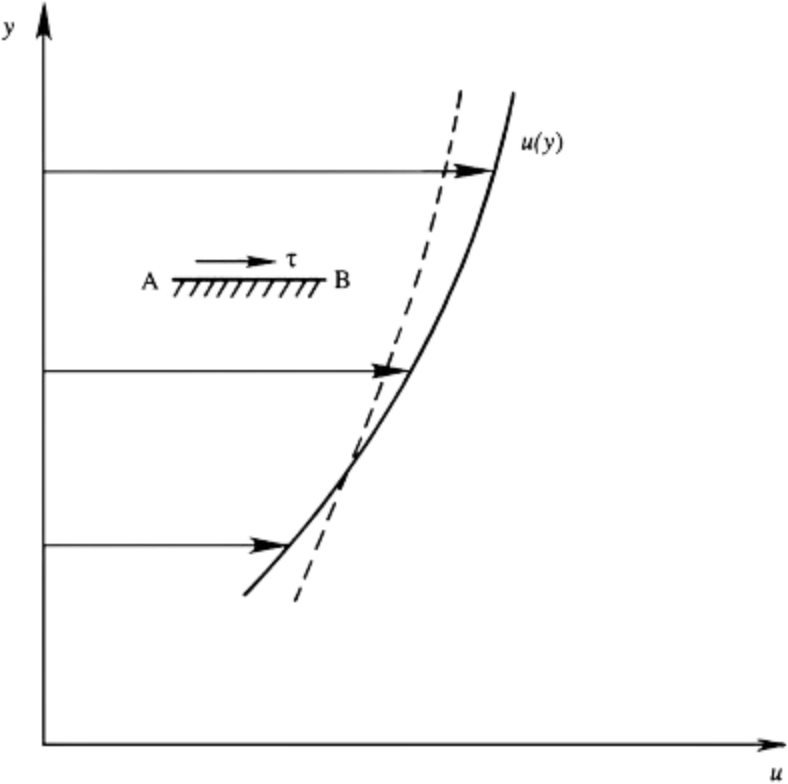
\includegraphics[width=0.5\textwidth]{img/N2_NS/Lecture1B_ShearStressSurfaceAB.png}
    \caption{This illustration shows how the shear stress $\tau$ in a fluid is approximately proportional to the velocity gradient.}
    \label{fig:N2_NS_shear_stress_proportionality}
\end{figure}
Fig. \ref{fig:N2_NS_shear_stress_proportionality} shows how the magnitude of the shear stress $\tau$ in a fluid depends on the velocity gradient. It has been shown experimentally that $\tau$ is approximately proportional to the velocity gradient, and that the proportionality factor is the \textit{dynamic viscosity} $\mu$
\begin{align}
	\tau = \mu \nabla \mathbf{u}
\end{align}
This is the definition of a \textit{Newtonian Fluid}. We can gain more insight by considering the sum $T_{ii}$
\begin{align}
	T_{ii} &= - 3p + 2 \mu S_{ii} + 3 \lambda S_{mm} \\
	&= - 3p + (2 \mu + 3 \lambda) \nabla \cdot \mathbf{u}
\end{align}
This implies that
\begin{align}
	p = -\frac{1}{3}T_{ii} + \left(\frac{2}{3} \mu + \lambda\right) \nabla \cdot \mathbf{u} \label{eq:N2_NS_pressure_stress_relation}
\end{align}
Now we define the mean pressure as the pressure in absence of shear and stress forces $\bar{p} = - \frac{1}{3} T_{ii}$ and substitute this into (\ref{eq:N2_NS_pressure_stress_relation}) to obtain
\begin{align}
	p - \bar{p} = \mu_v\nabla \cdot \mathbf{u}
\end{align}
Where we've introduced the \textit{coefficient of bulk viscosity} $\mu_v = \frac{2}{3} \mu + \lambda$. \textit{Stokes assumption} assumes that $\mu_v = 0$ such that $p = \bar{p}$. This is often a good assumption, since $\mu_v$ or $\nabla \cdot \mathbf{u}$ tend to be small for most flows.

\subsubsection{The Constitutive Equation}
Without Stokes assumption, the stress tensor is
\begin{align}
	T_{ij} &= -p \delta_{ij} + \tau_{ij} \\
	&= - p \delta_{ij} + 2\mu \left(S_{ij} - \frac{1}{3}S_{mm}\delta_{ij}\right) + \mu_v S_{mm}\delta){ij} \label{eq:N2_NS_constitutive_eq_newtonian}
\end{align}
This is the constitutive equation for a Newtonian fluid. If the fluid is incompressible, $S_{mm} = \nabla \cdot \mathbf{u} = 0$, so the constitutive equation reduces to
\begin{align}
	T_{ij} = - p \delta_{ij} + 2\mu S_{ij}
\end{align}

\subsubsection{Non-Newtonian fluid}
Add the constitutive equation for a non-Newtonian fluid here.

\subsection{The Navier-Stokes Momentum equation}
To obtain a momentum-conservation equation for a Newtonian fluid, we substitute the constitutive equation (\ref{eq:N2_NS_constitutive_eq_newtonian}) into Cauchy's equation of motion (\ref{eq:N2_NS_cauchy_equation_of_motion})
\begin{align}
	\rho \frac{D u_j}{D t} &= \rho g_j + \partial_i T_{ij} \\
	&= \rho g_j - \partial_i p + \partial_i \left[ 2 \mu S_{ij} - \frac{2}{3} \mu S_{mm} \delta_{ij} + \mu_v S_{mm} \delta_{ij} \right] \\
	&= \rho g_j - \partial_i p + \partial_i \left[ \mu (\partial_i u_j + \partial_j u_i) + \left(\mu_v - \frac{2}{3}\mu \right) \partial_m u_m \delta_{ij} \right] \label{eq:N2_NS_navier_stokes_compressible}
\end{align}
Eq. (\ref{eq:N2_NS_navier_stokes_compressible}) is called the \textit{Navier-Stokes momentum equation} or simply the Navier-Stokes equation. When the temperature differences are small within the flow, $\mu$ and $\mu_v$ can be regarded as locally constant, which allows us to write
\begin{align}
	\rho \frac{D u_j}{D t} &= \rho g_j - \partial_i p + \mu \partial_i^2 u_j + \mu \partial_j \partial_i u_i + \left(\mu_v - \frac{2}{3}\mu \right) \partial_i \partial_m u_m \delta_{ij} \\
	&= \rho g_j - \partial_i p + \mu \partial_i^2 u_j + \left(\mu_v + \frac{1}{3} \mu \right) \partial_j \partial_m u_m
\end{align}
This equation applies to compressible flow. For incompressible fluids $S_{mm} = 0$, so
\begin{align}
		\rho \frac{D u_j}{D t} &= \rho g_j - \partial_i p + \mu \partial_i^2 u_j
\end{align}
Or in vector notation
\begin{align}
	\rho \frac{D \mathbf{u}}{D t} &= \rho \mathbf{g} - \nabla p + \mu \nabla^2 \mathbf{u}
\end{align}
This is the Navier-Stokes equation for \textit{incompressible, Newtonian fluids}.

Note that the viscous term is related to the vorticity $\mathbf{\omega}$ in the following way
\begin{align}
	\mu \nabla^2 \mathbf{u} = - \mu \nabla \times \mathbf{\omega}
\end{align}
For inviscid flows, this term drops out. The resulting Navier-Stokes equation is called the \textit{Euler equation}
\begin{align}
	\rho \frac{D \mathbf{u}}{D t} &= \rho \mathbf{g} - \nabla p
\end{align}


\newpage
\section{Mathematical Interludes}

\end{document}